\documentclass[11pt]{article}
\usepackage[utf8]{inputenc}
\usepackage[T1]{fontenc}
\usepackage{amsmath}
\usepackage{amssymb}
\usepackage{multicol}
\usepackage{geometry}
\usepackage{tikz}
\usepackage{enumitem}
\usepackage{xcolor}
\usepackage{titlesec}

% Configurações de layout
\geometry{a4paper, left=1cm, right=1cm, top=0.5cm, bottom=1.2cm}
\setlength{\columnseprule}{0.4pt}

% Cores para títulos
\titleformat{\section}{\normalfont\Large\bfseries\color{blue}}{\thesection}{1em}{}
\titleformat{\subsection}{\normalfont\large\bfseries\color{red}}{\thesubsection}{1em}{}

% Comandos personalizados
\newcommand{\respostaNum}[1]{\textcolor{blue}{\boxed{#1}}}
\newcommand{\respostaTxt}[1]{\textcolor{blue}{#1}}
\newcommand{\resolucao}{\textbf{\textcolor{blue}{Resolução:}}}
\newcommand{\etapa}[1]{\textbf{\textcolor{red}{Etapa #1:}}}
\newcommand{\seta}{\textbf{\textcolor{green}{$\rightarrow$}}}

\title{\textcolor{red}{Gabarito Comentado: Medidas de Dispersão}}
\author{Professor: Jefferson}
\date{}

\begin{document}

\maketitle
\vspace{-1cm}

\begin{multicols}{2}

\section*{Instruções}
\textbf{Verifique suas respostas e estude as resoluções comentadas.}

\section*{Gabarito - Exercícios Básicos}

\begin{enumerate}[leftmargin=*]

\item \textbf{Calcule a amplitude dos conjuntos:}

\begin{enumerate}[label=\alph*)]
\item $4, 7, 9, 12, 18$

\resolucao

\textbf{\textcolor{red}{Etapa 1:}} Identificar o maior valor: $x_{\text{máx}} = 18$

\textbf{\textcolor{red}{Etapa 2:}} Identificar o menor valor: $x_{\text{mín}} = 4$

\textbf{\textcolor{red}{Etapa 3:}} Calcular a amplitude: $A = x_{\text{máx}} - x_{\text{mín}}$

\[
A = 18 - 4 = \respostaNum{14}
\]

\item $8, 8, 10, 12, 14, 18$

\resolucao

\textbf{\textcolor{red}{Etapa 1:}} $x_{\text{máx}} = 18$

\textbf{\textcolor{red}{Etapa 2:}} $x_{\text{mín}} = 8$

\textbf{\textcolor{red}{Etapa 3:}} $A = 18 - 8 = \respostaNum{10}$

\item $5, 10, 15, 20, 25, 30$

\resolucao

\textbf{\textcolor{red}{Etapa 1:}} $x_{\text{máx}} = 30$

\textbf{\textcolor{red}{Etapa 2:}} $x_{\text{mín}} = 5$

\textbf{\textcolor{red}{Etapa 3:}} $A = 30 - 5 = \respostaNum{25}$
\end{enumerate}

\item \textbf{Calcule a variância dos conjuntos:}

\begin{enumerate}[label=\alph*)]
\item $2, 4, 6, 8, 10$ (média = 6)

\resolucao

\textbf{\textcolor{red}{Etapa 1:}} Calcular cada desvio $(x_i - \bar{x})$:
\[2-6 = -4,\quad 4-6 = -2,\quad 6-6 = 0 \]
\[8-6 = 2,\quad 10-6 = 4\]

\textbf{\textcolor{red}{Etapa 2:}} Elevar cada desvio ao quadrado:
\[(-4)^2 = 16,\quad (-2)^2 = 4,\quad 0^2 = 0\]
\[ 2^2 = 4,\quad 4^2 = 16\]

\textbf{\textcolor{red}{Etapa 3:}} Somar os quadrados:
\[
16 + 4 + 0 + 4 + 16 = 40
\]

\textbf{\textcolor{red}{Etapa 4:}} Dividir pelo número de elementos ($n = 5$):
\[
Var = \frac{40}{5} = \respostaNum{8}
\]

\item $10, 10, 10, 10, 10$

\resolucao

\textbf{\textcolor{red}{Etapa 1:}} Todos os valores são iguais à média (10)

\textbf{\textcolor{red}{Etapa 2:}} Cada desvio é zero: $10-10 = 0$

\textbf{\textcolor{red}{Etapa 3:}} Quadrados dos desvios: $0, 0, 0, 0, 0$

\textbf{\textcolor{red}{Etapa 4:}} Soma = 0

\textbf{\textcolor{red}{Etapa 5:}} $Var = \frac{0}{5} = \respostaNum{0}$

\item $5, 8, 11, 14, 17$ (média = 11)

\resolucao

\textbf{\textcolor{red}{Etapa 1:}} Calcular cada desvio:
\[
5-11 = -6,\quad 8-11 = -3,\quad 11-11 = 0,\quad 14-11 = 3,\quad 17-11 = 6
\]

\textbf{\textcolor{red}{Etapa 2:}} Elevar ao quadrado:
\[
(-6)^2 = 36,\quad (-3)^2 = 9,\quad 0^2 = 0,\quad 3^2 = 9,\quad 6^2 = 36
\]

\textbf{\textcolor{red}{Etapa 3:}} Somar: $36 + 9 + 0 + 9 + 36 = 90$

\textbf{\textcolor{red}{Etapa 4:}} Dividir: $Var = \frac{90}{5} = \respostaNum{18}$
\end{enumerate}

\item \textbf{Calcule o desvio padrão dos conjuntos:}

\begin{enumerate}[label=\alph*)]
\item $1, 3, 5, 7, 9$ (variância = 10)

\resolucao

\textbf{\textcolor{red}{Etapa 1:}} Lembrar que $DP = \sqrt{Var}$

\textbf{\textcolor{red}{Etapa 2:}} $DP = \sqrt{10}$

\textbf{\textcolor{red}{Etapa 3:}} Calcular a raiz: $\sqrt{10} \approx \respostaNum{3,16}$

\item $20, 25, 30, 35, 40$ (variância = 50)

\resolucao

$DP = \sqrt{50} = \sqrt{25 \cdot 2} = 5\sqrt{2} \approx \respostaNum{7,07}$

\item $100, 102, 104, 106, 108$ (variância = 10)

\resolucao

$DP = \sqrt{10} \approx \respostaNum{3,16}$
\end{enumerate}

\item \textbf{Dado o conjunto: $5, 8, 8, 12, 15, 20$, calcule:}

\resolucao

\textbf{\textcolor{red}{Etapa 1:}} Calcular a média:
\[
\bar{x} = \frac{5 + 8 + 8 + 12 + 15 + 20}{6} = \frac{68}{6} \approx 11,33
\]

\begin{enumerate}[label=\alph*)]
\item Amplitude

\textbf{\textcolor{red}{Etapa 1:}} $x_{\text{máx}} = 20$, $x_{\text{mín}} = 5$

\textbf{\textcolor{red}{Etapa 2:}} $A = 20 - 5 = \respostaNum{15}$

\item Variância

\textbf{\textcolor{red}{Etapa 1:}} Calcular os desvios:
\[5-11,33 = -6,33,\quad 8-11,33 = -3,33 \] 
\[ 8-11,33 = -3,33, \quad 12-11,33 = 0,67 \]
\[15-11,33 = 3,67,\quad 20-11,33 = 8,67 \]

\textbf{\textcolor{red}{Etapa 2:}} Elevar ao quadrado:
\[(-6,33)^2 = 40,07,\quad (-3,33)^2 = 11,09\]
\[(-3,33)^2 = 11,09, \quad (0,67)^2 = 0,45 \]
\[ (3,67)^2 = 13,47,\quad (8,67)^2 = 75,17 \]

\textbf{\textcolor{red}{Etapa 3:}} Somar: $40,07 + 11,09 + 11,09 + 0,45 + 13,47 + 75,17 = 151,34$

\textbf{\textcolor{red}{Etapa 4:}} Dividir: $Var = \frac{151,34}{6} \approx \respostaNum{25,22}$

\item Desvio padrão

$DP = \sqrt{25,22} \approx \respostaNum{5,02}$

\item Coeficiente de variação

$CV = \frac{5,02}{11,33} \times 100\% \approx \respostaNum{44,3\%}$

\respostaTxt{Alta dispersão (CV > 30\%)}
\end{enumerate}

\item \textbf{Compare os conjuntos usando CV:}

\textbf{Conjunto A:} $\bar{x} = 2500$, $DP = 500$

\textbf{Conjunto B:} $\bar{x} = 25$, $DP = 5$

\begin{enumerate}[label=\alph*)]
\item Calcule o CV de cada conjunto

\resolucao

\textbf{Conjunto A:}

\textbf{\textcolor{red}{Etapa 1:}} Aplicar fórmula $CV = \frac{DP}{\bar{x}} \times 100\%$

\textbf{\textcolor{red}{Etapa 2:}} $CV_A = \frac{500}{2500} \times 100\% = 0,2 \times 100\% = \respostaNum{20\%}$

\textbf{Conjunto B:}

$CV_B = \frac{5}{25} \times 100\% = 0,2 \times 100\% = \respostaNum{20\%}$

\item Qual conjunto é mais homogêneo?

\respostaTxt{Ambos têm a mesma dispersão relativa (20\%)}
\end{enumerate}

\item \textbf{Problemas contextualizados:}

\begin{enumerate}[label=\alph*)]
\item Notas de João: 6, 7, 8, 9. Pedro: 4, 6, 8, 10.

\resolucao

\textbf{João:}

\textbf{\textcolor{red}{Etapa 1:}} Calcular a média:
\[
\bar{x}_J = \frac{6+7+8+9}{4} = \frac{30}{4} = 7,5
\]

\textbf{\textcolor{red}{Etapa 2:}} Calcular desvios:
\[6-7,5 = -1,5,\quad 7-7,5 = -0,5 \] 
\[8-7,5 = 0,5,\quad 9-7,5 = 1,5\]

\textbf{\textcolor{red}{Etapa 3:}} Quadrados:
\[
    (-1,5)^2 = 2,25,\quad (-0,5)^2 = 0,25 \] 
\[ (0,5)^2 = 0,25,\quad (1,5)^2 = 2,25 \]

\textbf{\textcolor{red}{Etapa 4:}} Somar: $2,25 + 0,25 + 0,25 + 2,25 = 5$

\textbf{\textcolor{red}{Etapa 5:}} Variância: $Var_J = \frac{5}{4} = 1,25$

\textbf{\textcolor{red}{Etapa 6:}} Desvio padrão: $DP_J = \sqrt{1,25} \approx \respostaNum{1,12}$

\textbf{Pedro:}

\textbf{\textcolor{red}{Etapa 1:}} Média: $\bar{x}_P = \frac{4+6+8+10}{4} = \frac{28}{4} = 7$

\textbf{\textcolor{red}{Etapa 2:}} Desvios: $4-7 = -3,\quad 6-7 = -1,\quad 8-7 = 1,\quad 10-7 = 3$

\textbf{\textcolor{red}{Etapa 3:}} Quadrados: $9, 1, 1, 9$

\textbf{\textcolor{red}{Etapa 4:}} Soma: $9+1+1+9 = 20$

\textbf{\textcolor{red}{Etapa 5:}} Variância: $Var_P = \frac{20}{4} = 5$

\textbf{\textcolor{red}{Etapa 6:}} Desvio padrão: $DP_P = \sqrt{5} \approx \respostaNum{2,24}$

\textbf{Comparação:} $1,12 < 2,24$

\respostaTxt{João tem desempenho mais regular (menor DP)}

\item Duas turmas: Turma A $DP = 1,2$, Turma B $DP = 2,5$

\resolucao

\textbf{\textcolor{red}{Etapa 1:}} Comparar os desvios padrão

\textbf{\textcolor{red}{Etapa 2:}} $1,2 < 2,5$

\respostaTxt{Turma A é mais homogênea (menor dispersão)}
\end{enumerate}

\item \textbf{Calcule todas as medidas de dispersão para:}

\begin{enumerate}[label=\alph*)]
\item $10, 20, 30, 40, 50$

\resolucao

\textbf{\textcolor{red}{Etapa 1:}} Calcular a média
\[
\bar{x} = \frac{10 + 20 + 30 + 40 + 50}{5} = \frac{150}{5} = 30
\]

\textbf{\textcolor{red}{Etapa 2:}} Calcular amplitude
\[
A = 50 - 10 = 40
\]

\textbf{\textcolor{red}{Etapa 3:}} Calcular desvios
\[
10-30 = -20,\quad 20-30 = -10,\quad 30-30 = 0,\quad 40-30 = 10,\quad 50-30 = 20
\]

\textbf{\textcolor{red}{Etapa 4:}} Quadrados dos desvios
\[
400,\quad 100,\quad 0,\quad 100,\quad 400
\]

\textbf{\textcolor{red}{Etapa 5:}} Somar os quadrados
\[
400 + 100 + 0 + 100 + 400 = 1000
\]

\textbf{\textcolor{red}{Etapa 6:}} Calcular variância
\[
Var = \frac{1000}{5} = 200
\]

\textbf{\textcolor{red}{Etapa 7:}} Calcular desvio padrão
\[
DP = \sqrt{200} = 10\sqrt{2} \approx 14,14
\]

\textbf{\textcolor{red}{Etapa 8:}} Calcular coeficiente de variação
\[
CV = \frac{14,14}{30} \times 100\% \approx 47,1\%
\]

\respostaNum{40},\quad \respostaNum{200},\quad \respostaNum{14,14},\quad \respostaNum{47,1\%}

\item $5, 5, 5, 5, 5, 5$

\resolucao

\textbf{\textcolor{red}{Etapa 1:}} Média $\bar{x} = 5$

\textbf{\textcolor{red}{Etapa 2:}} Amplitude $A = 5 - 5 = 0$

\textbf{\textcolor{red}{Etapa 3:}} Todos os desvios são zero $\rightarrow$ $Var = 0$

\textbf{\textcolor{red}{Etapa 4:}} $DP = 0$

\textbf{\textcolor{red}{Etapa 5:}} $CV = 0\%$

\respostaNum{0},\quad \respostaNum{0},\quad \respostaNum{0},\quad \respostaNum{0\%}

\item $15, 16, 17, 18, 19, 20$

\resolucao

\textbf{\textcolor{red}{Etapa 1:}} Média $\bar{x} = \frac{105}{6} = 17,5$

\textbf{\textcolor{red}{Etapa 2:}} Amplitude $A = 20 - 15 = 5$

\textbf{\textcolor{red}{Etapa 3:}} Desvios:
\[
-2,5,\quad -1,5,\quad -0,5,\quad 0,5,\quad 1,5,\quad 2,5
\]

\textbf{\textcolor{red}{Etapa 4:}} Quadrados:
\[
6,25,\quad 2,25,\quad 0,25,\quad 0,25,\quad 2,25,\quad 6,25
\]

\textbf{\textcolor{red}{Etapa 5:}} Soma: $6,25 + 2,25 + 0,25 + 0,25 + 2,25 + 6,25 = 17,5$

\textbf{\textcolor{red}{Etapa 6:}} Variância: $Var = \frac{17,5}{6} \approx 2,92$

\textbf{\textcolor{red}{Etapa 7:}} Desvio padrão: $DP = \sqrt{2,92} \approx 1,71$

\textbf{\textcolor{red}{Etapa 8:}} Coeficiente de variação: $CV = \frac{1,71}{17,5} \times 100\% \approx 9,77\%$

\respostaNum{5},\quad \respostaNum{2,92},\quad \respostaNum{1,71},\quad \respostaNum{9,77\%}
\end{enumerate}

\item \textbf{Analise os conjuntos:}

\textbf{Conjunto X:} $100, 102, 104, 106, 108, 110$

\textbf{Conjunto Y:} $0, 10, 20, 30, 40, 50$

\begin{enumerate}[label=\alph*)]
\item Amplitude de cada

\resolucao

\textbf{Conjunto X:} $A_X = 110 - 100 = \respostaNum{10}$

\textbf{Conjunto Y:} $A_Y = 50 - 0 = \respostaNum{50}$

\item Desvio padrão de cada

\resolucao

\textbf{Conjunto X:}

\textbf{\textcolor{red}{Etapa 1:}} Média $\bar{x}_X = \frac{630}{6} = 105$

\textbf{\textcolor{red}{Etapa 2:}} Desvios: $-5, -3, -1, 1, 3, 5$

\textbf{\textcolor{red}{Etapa 3:}} Quadrados: $25, 9, 1, 1, 9, 25$

\textbf{\textcolor{red}{Etapa 4:}} Soma: $25+9+1+1+9+25 = 70$

\textbf{\textcolor{red}{Etapa 5:}} Variância: $Var_X = \frac{70}{6} \approx 11,67$

\textbf{\textcolor{red}{Etapa 6:}} $DP_X = \sqrt{11,67} \approx \respostaNum{3,42}$

\textbf{Conjunto Y:}

\textbf{\textcolor{red}{Etapa 1:}} Média $\bar{x}_Y = \frac{150}{6} = 25$

\textbf{\textcolor{red}{Etapa 2:}} Desvios: $-25, -15, -5, 5, 15, 25$

\textbf{\textcolor{red}{Etapa 3:}} Quadrados: $625, 225, 25, 25, 225, 625$

\textbf{\textcolor{red}{Etapa 4:}} Soma: $625+225+25+25+225+625 = 1750$

\textbf{\textcolor{red}{Etapa 5:}} Variância: $Var_Y = \frac{1750}{6} \approx 291,67$

\textbf{\textcolor{red}{Etapa 6:}} $DP_Y = \sqrt{291,67} \approx \respostaNum{17,08}$

\item Coeficiente de variação

\resolucao

$CV_X = \frac{3,42}{105} \times 100\% \approx \respostaNum{3,26\%}$

$CV_Y = \frac{17,08}{25} \times 100\% \approx \respostaNum{68,32\%}$

\item Compare a variabilidade relativa

\respostaTxt{Conjunto X é muito mais homogêneo (3,26\% < 68,32\%)}
\end{enumerate}

\item \textbf{Dado o conjunto: $3, 7, 11, 15, 19$}

\begin{enumerate}[label=\alph*)]
\item Média

\resolucao

$\bar{x} = \frac{3+7+11+15+19}{5} = \frac{55}{5} = \respostaNum{11}$

\item Desvios $(x_i - \bar{x})$

\resolucao

$3-11 = \respostaNum{-8},\quad 7-11 = \respostaNum{-4},\quad 11-11 = \respostaNum{0},\quad 15-11 = \respostaNum{4},\quad 19-11 = \respostaNum{8}$

\item Variância

\resolucao

\textbf{\textcolor{red}{Etapa 1:}} Quadrados: $64, 16, 0, 16, 64$

\textbf{\textcolor{red}{Etapa 2:}} Soma: $64+16+0+16+64 = 160$

\textbf{\textcolor{red}{Etapa 3:}} $Var = \frac{160}{5} = \respostaNum{32}$

\item Desvio padrão

\resolucao

$DP = \sqrt{32} = \sqrt{16 \cdot 2} = \respostaNum{4\sqrt{2} \approx 5,66}$
\end{enumerate}

\item \textbf{Exercício de interpretação:}

\begin{enumerate}[label=\alph*)]
\item Se $DP = 0$, o que podemos afirmar?

\resolucao

\textbf{\textcolor{red}{Etapa 1:}} $DP = 0 \Rightarrow \sqrt{Var} = 0 \Rightarrow Var = 0$

\textbf{\textcolor{red}{Etapa 2:}} $Var = 0 \Rightarrow$ todos os desvios são zero

\textbf{\textcolor{red}{Etapa 3:}} Todos os valores são iguais à média

\respostaTxt{Todos os dados são iguais (dispersão nula)}

\item Amplitude zero e $DP \neq 0$?

\resolucao

\textbf{\textcolor{red}{Etapa 1:}} Amplitude zero $\Rightarrow x_{\text{máx}} = x_{\text{mín}}$

\textbf{\textcolor{red}{Etapa 2:}} Se todos valores são iguais, $DP = 0$

\respostaTxt{Não é possível}

\item Medida mais sensível a valores extremos

\resolucao

\textbf{\textcolor{red}{Análise:}} A amplitude usa apenas os valores extremos

\textbf{\textcolor{red}{Conclusão:}} A amplitude é mais sensível

\respostaTxt{Amplitude é mais sensível a valores extremos}
\end{enumerate}
\end{enumerate}

\section*{Gabarito - Exercícios Avançados}

\begin{enumerate}[leftmargin=*, start=11]

\item \textbf{Duas empresas:}

Empresa A: $\bar{x} = 3000$, $DP = 600$

Empresa B: $\bar{x} = 5000$, $DP = 800$

\resolucao

\textbf{\textcolor{red}{Etapa 1:}} Calcular CV da Empresa A
\[
CV_A = \frac{600}{3000} \times 100\% = 0,2 \times 100\% = 20\%
\]

\textbf{\textcolor{red}{Etapa 2:}} Calcular CV da Empresa B
\[
CV_B = \frac{800}{5000} \times 100\% = 0,16 \times 100\% = 16\%
\]

\textbf{\textcolor{red}{Etapa 3:}} Comparar: $16\% < 20\%$

\respostaTxt{Empresa B tem menor dispersão relativa (16\% < 20\%)}

\item \textbf{Dados agrupados:}

\begin{center}
\begin{tabular}{|c|c|c|c|c|}
\hline
Notas & $x_i$ & $f_i$ & $x_i \cdot f_i$ & $(x_i - \bar{x})^2 \cdot f_i$ \\
\hline
0-2 & 1 & 2 & 2 & 37,32 \\
2-4 & 3 & 5 & 15 & 26,91 \\
4-6 & 5 & 8 & 40 & 0,82 \\
6-8 & 7 & 10 & 70 & 28,22 \\
8-10 & 9 & 5 & 45 & 67,71 \\
\hline
Total & & 30 & 172 & 160,98 \\
\hline
\end{tabular}
\end{center}

\begin{enumerate}[label=\alph*)]
\item Média

\resolucao

$\bar{x} = \frac{172}{30} \approx \respostaNum{5,73}$

\item Desvio padrão

\resolucao

\textbf{\textcolor{red}{Etapa 1:}} Variância: $Var = \frac{160,98}{30} \approx 5,37$

\textbf{\textcolor{red}{Etapa 2:}} $DP = \sqrt{5,37} \approx \respostaNum{2,32}$

\item Coeficiente de variação

\resolucao

$CV = \frac{2,32}{5,73} \times 100\% \approx \respostaNum{40,5\%}$

\respostaTxt{Alta dispersão (CV > 30\%)}
\end{enumerate}

\item \textbf{Tabela completa:}

Dados: $4, 6, 8, 10, 12$

\resolucao

\textbf{\textcolor{red}{Etapa 1:}} Média $\bar{x} = \frac{40}{5} = 8$

\begin{center}
\begin{tabular}{|c|c|c|c|}
\hline
$x_i$ & $x_i - \bar{x}$ & $(x_i - \bar{x})^2$ & $x_i^2$ \\
\hline
4 & -4 & 16 & 16 \\
6 & -2 & 4 & 36 \\
8 & 0 & 0 & 64 \\
10 & 2 & 4 & 100 \\
12 & 4 & 16 & 144 \\
\hline
Soma & 0 & 40 & 360 \\
\hline
\end{tabular}
\end{center}

\textbf{Variância fórmula padrão:}
\[
Var = \frac{40}{5} = \respostaNum{8}
\]

\textbf{Variância fórmula alternativa:}
\[
Var = \frac{360}{5} - 8^2 = 72 - 64 = \respostaNum{8}
\]

\item \textbf{Dois produtos:}

Produto X: R\$ 50, $DP = 5$

Produto Y: R\$ 200, $DP = 20$

\resolucao

\textbf{\textcolor{red}{Etapa 1:}} $CV_X = \frac{5}{50} \times 100\% = 10\%$

\textbf{\textcolor{red}{Etapa 2:}} $CV_Y = \frac{20}{200} \times 100\% = 10\%$

\respostaTxt{Ambos têm a mesma estabilidade relativa (10\%)}
\end{enumerate}

\section*{Resumo das Fórmulas}

\begin{center}
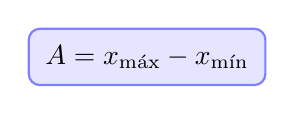
\begin{tikzpicture}
\node[rectangle, fill=blue!10, rounded corners, inner sep=6pt, draw=blue!50, thick] (box) {
$\displaystyle A = x_{\text{máx}} - x_{\text{mín}}$
};
\end{tikzpicture}

\vspace{0.2cm}

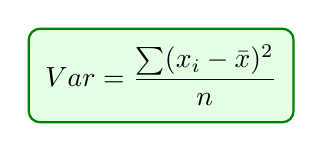
\begin{tikzpicture}
\node[rectangle, fill=green!10, rounded corners, inner sep=6pt, draw=green!50!black, thick] (box) {
$\displaystyle Var = \frac{\sum (x_i - \bar{x})^2}{n}$
};
\end{tikzpicture}

\vspace{0.2cm}

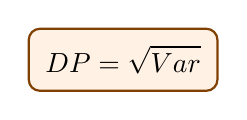
\begin{tikzpicture}
\node[rectangle, fill=orange!10, rounded corners, inner sep=6pt, draw=orange!50!black, thick] (box) {
$\displaystyle DP = \sqrt{Var}$
};
\end{tikzpicture}

\vspace{0.2cm}

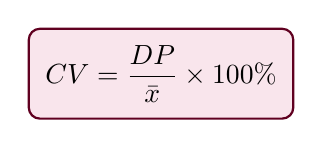
\begin{tikzpicture}
\node[rectangle, fill=purple!10, rounded corners, inner sep=6pt, draw=purple!50!black, thick] (box) {
$\displaystyle CV = \frac{DP}{\bar{x}} \times 100\%$
};
\end{tikzpicture}
\end{center}

\vspace{0.3cm}
\textcolor{blue}{\textbf{Legenda:}} 
\begin{itemize}
\item \textcolor{blue}{Respostas numéricas:} \respostaNum{exemplo}
\item \textcolor{blue}{Respostas textuais:} \textcolor{blue}{exemplo}
\end{itemize}

\vspace{0.3cm}
\textcolor{red}{\textbf{Classificação do CV:}}
\begin{itemize}
\item \textcolor{blue}{CV < 15\%:} Baixa dispersão
\item \textcolor{blue}{15\% ≤ CV ≤ 30\%:} Média dispersão
\item \textcolor{blue}{CV > 30\%:} Alta dispersão
\end{itemize}

\end{multicols}

\end{document}
